\documentclass[submit]{harvardml}

% Put in your full name and email address.
\name{Jazz Zhao}
\email{jzhao@college.harvard.edu}

% List any people you worked with.
\collaborators{%
    N/A
}

% You don't need to change these.
\course{CS51}
\assignment{Final Project}
\duedate{5pm May 2, 2018} 
\usepackage{listings}
\usepackage{common}
\usepackage{float}
\usepackage{graphicx}
\usepackage[mmddyyyy,hhmmss]{datetime}
\usepackage{color}
\definecolor{dkgreen}{rgb}{0,0.6,0}
\definecolor{gray}{rgb}{0.5,0.5,0.5}
\definecolor{mauve}{rgb}{0.58,0,0.82}

\lstset{frame=tb,
	language=[Objective]{Caml},
	aboveskip=3mm,
	belowskip=3mm,
	showstringspaces=false,
	columns=flexible,
	basicstyle={\small\ttfamily},
	numbers=none,
	numberstyle=\tiny\color{gray},
	keywordstyle=\color{blue},
	commentstyle=\color{dkgreen},
	stringstyle=\color{mauve},
	breaklines=true,
	breakatwhitespace=true,
	tabsize=3
}


\begin{document}
\begin{center}
{\Large MiniML Writeup}\\
\end{center}

\subsection*{Introduction}
I decided to implement the suggested extension, that is, an additionally evaluation function which evaluates expressions using the environment model and lexical scoping, as compared to the standard dynamically scoped environment model.

\subsection*{Difference between dynamic and lexical scope}

In the dynamically scoped environment model implemented in eval\_d, expressions are evaluated within the dynamic application environment. For example, the following demonstrates the state of the environment after each line of code (as comments) under dynamic scope, where the entire expression evaluates to 5. (Example from lecture 13)
\begin{lstlisting}
let x = 1 in (* [x -> 1] *)
let f =
	fun y -> x + y in (* [x -> 1; f -> fun y -> x + y] *)
let x = 2 in (* [x -> 2; f -> fun y -> x + y] *)
f 3 ;; (* [x -> 2; f -> fun y -> x + y; y -> 3] *)
= 5
\end{lstlisting}

However, if we type this expression into utop, we see that it evaluates to 4 instead due to the different scope: Under lexical scope, the variable $x$ takes its value not from the last let statement before the function call but the let statement before the function definition. 

As seen in lecture 13, we can save a snapshot of the environment at the time of the function definition with the function value itself using closures, which pair a function with its lexical environment:
\begin{lstlisting}
let x = 1 in (* [x -> 1] *)
let f =
	fun y -> x + y in (* [x -> 1; f -> (fun y -> x + y, [x -> 1])] *)
let x = 2 in (* [x -> 2; f -> (fun y -> x + y, [x -> 1])]*)
f 3 ;; (* [x -> 2;f -> (fun y -> x + y, [x -> 1]); y -> 3] *)
= 4
\end{lstlisting}

Then, at the time when we evaluate the function applied to 3, we evaluate it in the environment that we saved in the closure where [x $\rightarrow$ 1] rather than [x $\rightarrow$ 2], which evaluates to 1 + 3 = 4.

\subsection*{Implementation}
I implemented the lexically scoped environment model as eval\_l, which shares most of its code with eval\_d (and a significant portion with eva\_s too). I thus decided to implement a general function evaluate that is partially applied in order to create the different evaluation functions.

In particular, there are only 2 different cases between eval\_d and eval\_l shown below:

\begin{itemize}
	\item \textbf{Function Definitions:} Under the substitution model and the dynamic scope model, functions simply evaluate to themselves. In eval\_l however, functions will evaluate to a closure of the function itself and the current (definition) environment.
	\begin{lstlisting}
	let rec evaluate (substitution : bool)
						    (dynamic : bool)
							 (exp : expr)
							 (env : Env.env)
							: Env.value =
							
		let open Env in
		
		(* eval function that takes an environment *)
		let eval = evaluate substitution dynamic in
		
		(* eval that ignores invironment, e.g. for substitution model *)
		let eval' exp = eval exp env in
		
		(* returns error with given string *)
		let oops (str : string) =
			raise (EvalError str) in
		
		(* returns evaluated expression as expr instead of as Env.value *)
		let eval_to_exp (value : expr) : expr =
			match eval' value with
			| Val exp -> exp
			| _ -> oops "Type Error" in
			
		(* where the actual evaluation will take place *)
		match exp with
		...
		| Fun _ -> if substitution || dynamic then Val exp
		else close exp env
		...
	\end{lstlisting}
	\item \textbf{Function Applications:} Under both models, we first evaluate the first argument, which must be a function value, since non-functions cannot be applied.
	
	Then, under the dynamically scoped model, we extend the environment to have the value of the function point to the evaluated function argument (i.e. app), and evaluate the definition of the function in this new environment. Going back to our example, this would correspond to first adding [y $\rightarrow$ 3] to our environment, and then evaluating x + y (i.e. the function definition) in our new environment.
	
	Under the lexically scoped environment, we essentially go through the same process with one crucial difference: rather than using the current environment, we use the environment stored at the time of the function definition, i.e. env' instead of env.

	\begin{lstlisting}
		... (* continuing the code from above *)
		| App (f, app) ->    if substitution then
									  ...
									else if dynamic then
										(match eval_to_exp f with
										  | Fun (x, def) -> eval def (extend env x (ref (eval' app)))
										  | _ -> oops "Nonfunction bcannot be applied")
									else
										(match eval' f with
										  | Closure (Fun (x, def), env') -> eval def (extend env' x (ref (eval' app)))
										  | _ -> oops "Nonfunction ccannot be applied")
    ;;
	\end{lstlisting}
\end{itemize}

\subsection*{Demonstration}
When evaluate is set to eval\_d:
\begin{figure}[H]
	\centering
	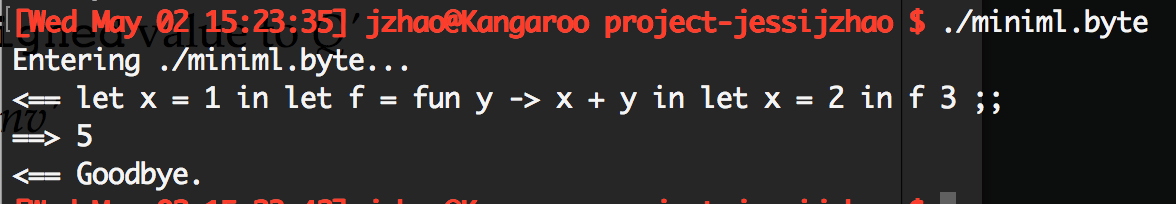
\includegraphics[width=300 pt]{dynamic}
\end{figure}

When evaluate is set to eval\_l:
\begin{figure}[H]
	\centering
	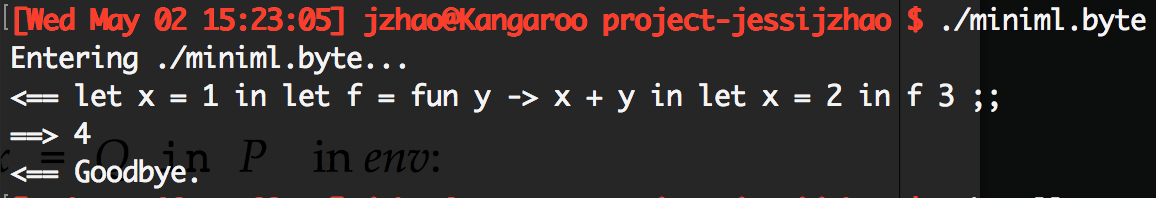
\includegraphics[width=300 pt]{lexical}
\end{figure}



\end{document}
